\section{Related Work}
\label{sec:method}

\subsection{Text-Based LLM Interfaces}
Since the introduction of the Transformer architecture in "Attention Is All You Need", text-based content generation and processing have become the central foundation of modern natural language processing (NLP).\cite{vaswani2017attention}
In this context, large language models are a family of neural language models trained on vast amounts of textual data and capable of performing a wide range of natural language processing tasks, such as generating context-aware responses based on user-provided text prompts.\cite{brown2020language}
To utilize this family of models as a user interface, the model must be capable of understanding domain-specific context and of acting upon user prompts, rather than merely generating textual responses. 
Several methods exist to enable this, a brief summary of these approaches is provided below.

\subsubsection{Fine Tuning}
Fine-tuning is the process of further training a pre-trained model on task- or domain-specific data by updating its existing parameters or, in some approaches, by introducing additional trainable parameters.\cite{mosbach2023analyzing}
By further training the model on a domain-specific dataset, for example technical data on extraterrestrial habitats, a base model such as GPT-5 can acquire contextual knowledge of the application domain and generate its responses accordingly.

However, a significant downside of this approach is the increased risk of model hallucinations. Hallucinations refer to the phenomenon in which a model generates incorrect or fabricated information in response to a given prompt.\cite{gekhman2024fine}
Such behavior can pose a significant risk in safety-critical environments.

\subsubsection{Retrieval Augmented Generation}
Retrieval-Augmented Generation (RAG) introduces relevant external information to the language model without modifying the model’s internal parameters.

\begin{figure}[h]
    \centering
    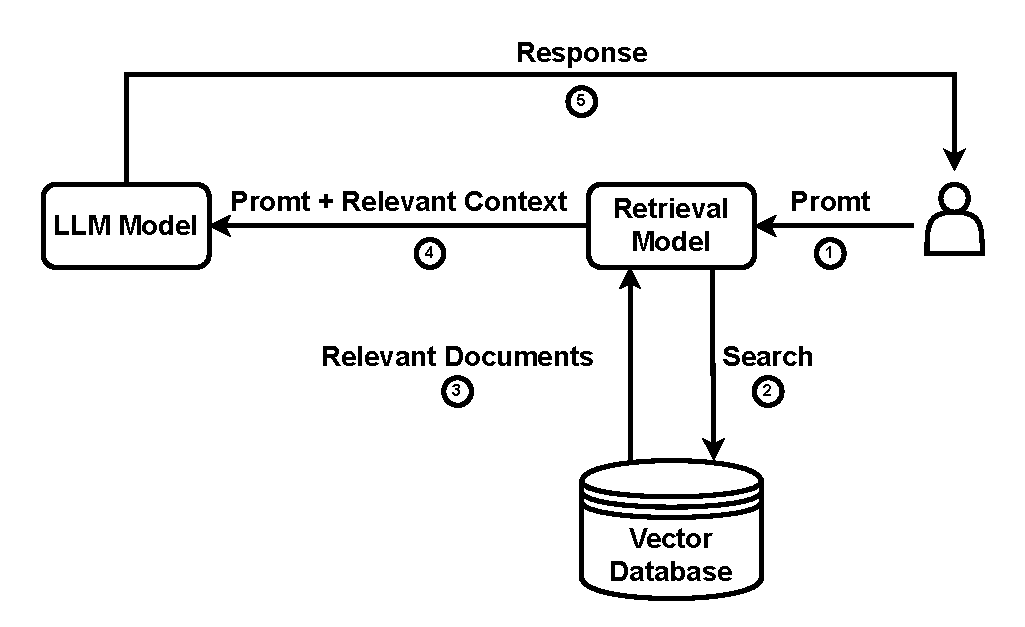
\includegraphics[width=0.8\linewidth]{bilder/RAG.pdf}
    \caption{High-level RAG workflow that injects retrieved documents into the prompt instead of altering model weights.}
    \label{fig:rag_workflow}
\end{figure}

As shown in Figure \ref{fig:rag_workflow}, the RAG workflow begins with a user prompt; however, instead of passing the prompt directly to the LLM, a similarity search is first performed over context-relevant information stored as embeddings in a vector database. The retrieved context is then provided together with the prompt to the LLM for grounded response generation.\cite{brown2020language}
Recent studies have shown this to be a more reliable method for context retrieval compared to fine-tuning.\cite{ovadia2024finetuning}
However the risk of hallucinations even with RAG is still a non zero possibility. However with good 
\subsubsection{Tool Use / Function Calling}

\subsubsection{Agent Architectures}


\subsection{Speech-to-Text, LLM and Text-to-Speech}
A large body of systems research still follows the classic speech-to-text pipeline: incoming speech is transcribed, processed by an LLM, and subsequently rendered back to audio through text-to-speech engines. This architecture remains attractive because the intermediate textual representation makes it straightforward to integrate retrieval, grounding, or enterprise knowledge bases, even though the multi-stage pipeline can add noticeable latency.

\subsection{Speech-to-Speech LLMs}
Recent work on speech-native LLMs, popularized by OpenAI's realtime models, reduces the round-trip delay by operating directly on streaming audio chunks. The model begins producing speech tokens almost immediately, providing near-realtime turn-taking during conversations. These systems trade some reasoning depth compared with larger text-first models such as GPT-4o or GPT-5, and incorporating retrieval-augmented generation is still an active research topic, but they mark the state of the art for responsive spoken interactions.

\subsection{Vision-Language(-Action) Models}
Vision-language(-action) models extend LLM capabilities to video feeds, sensor data, and embodied decision making. They process multimodal streams to ground language in the physical environment and to suggest or execute actions. Although still nascent, this strand of work is highly relevant for human-machine interaction scenarios that require situational awareness or co-robotic collaboration.
